
\documentclass[11pt]{article}

\usepackage{graphicx}
\usepackage{float}
\usepackage{amssymb}
\usepackage{amsmath}
\usepackage{amsthm}
\usepackage{amsfonts}
\usepackage{enumitem}
\usepackage{pdfpages}
\usepackage[margin=1in]{geometry}

\newenvironment{solution}
  {\par\noindent\textbf{Solution:}\par}
  {\par}

\renewcommand{\thesubsection}{(\alph{subsection})}
\renewcommand{\thesection}{\arabic{section}} % Keeps section numbering as 1, 2, 3...

\usepackage{etoolbox} % Required for \pretocmd
\pretocmd{\section}{\setcounter{subsection}{0}}{}{}

\title{MATH 340, 2024/25, Term 2, Assignment 3}
\author{Mercury Mcindoe 85594505} 

\begin{document}
\maketitle 
\thispagestyle{empty}

\section*{Question 1}
\subsection{}
\begin{solution}
  Let's assume $\textbf{z},\textbf{w} \in F$ such that $\textbf{z}=A\textbf{u} \le \textbf{b}, \textbf{w}=A\textbf{v} \le \textbf{b}$ where $\exists \textbf{u},\textbf{v} \in \mathbb{R}^n$ and $\textbf{u},\textbf{v} \ge \mathbf{0}$.
  Let $t \in [0,1]$ and let's also look at $(1-t)\textbf{z} + t\textbf{w}$,
  \[
    (1-t)\textbf{z}+t\textbf{w}= (1-t)(A\textbf{u}) + t(A\textbf{v}) 
  \]
  Also, since $t \in [0,1]$ we can see that $(1-t)\textbf{z},t\textbf{w}\ge \textbf{0} \to (1-t)\textbf{z} + t\textbf{w} \ge \textbf{0}$.
  Since we know that $t\in[0,1]$ as well as $\textbf{u},\textbf{v} \ge \mathbf{0}$ we can also conclude that the following,
  \[
    (1-t)(A\textbf{u}) \le (1-t)\textbf{b} \text{ and } t(A\textbf{v}) \le t\textbf{b} 
  \]
  Therefore,
  \[
    (1-t)\textbf{z} + t\textbf{w} = (1-t)(A\textbf{u}) + t(A\textbf{v}) \le (1-t)\textbf{b} + t\textbf{b} = \textbf{b}
  \]
  showing that $(1-t)\textbf{z} + t\textbf{w} \in F$ hence $F$ is convex.
\end{solution}

\subsection{}
\begin{solution}
  Let's first show that $\lambda\textbf{u} + (1-\lambda)\textbf{v}$ is a feasible solution to the LP. Since we know that $\lambda \in [0,1]$ and $\textbf{u},\textbf{v} \ge \textbf{0}$, we have that 
  \[
    \lambda \textbf{u} + (1-\lambda)\textbf{v} \ge \textbf{0}
  \]
  Also, we showed from (a) that the set $\left\{ \textbf{x}\in \mathbb{R}^n \hspace{.05in} \vert \hspace{.05in} A\textbf{x} \ge \textbf{b}, \quad \textbf{x} \ge \textbf{0} \right\}$ is convex. Hence,
    $\lambda \textbf{u} + (1-\lambda)\textbf{v}$ is in the feasible region. Making $\lambda\textbf{u} + (1-\lambda)\textbf{v}$ a feasible solution. \\  \\
    Now, let's show that $\lambda \textbf{u} + (1-\lambda)\textbf{v}$ has the same value of the objective function as $\textbf{u}$. Since $\textbf{u}$ is an optimal solution, let's denote $\textbf{c} \cdot \textbf{u}$ as $\alpha_\text{max}$ 
    Then, $\textbf{c} \cdot \textbf{v} = \alpha_\text{max}$ as well.
    \[
      \begin{aligned}
        \textbf{c} \cdot (\lambda \textbf{u} + (1-\lambda)\textbf{v}) &= \lambda (\textbf{c} \cdot \textbf{u}) + (1-\lambda)(\textbf{c} \cdot \textbf{v}) \\ 
                                                                      &= \lambda (\alpha_{\text{max}}) + (1-\lambda)(\alpha_\text{max}) \\ 
                                                                      &= \alpha_\text{max} \\ 
                                                                      &= \textbf{c} \cdot \textbf{u}
      \end{aligned}
    \]
    as required.
  \end{solution}

\section*{Question 2}
\subsection{}
\begin{solution}
  No it is \textbf{not} true that every linear programming problem has an optimal solution. Let's consider this example,
  \[
    \begin{aligned}
      \text{maximize } &x_0 + x_1 \\ 
      \text{subject to } &2x_0 + x_1 \ge 2 \\ 
                        &x_0 +2x_1 \ge 2 \\ 
                        &x_0,x_1 \ge 0
    \end{aligned}
  \]
  If we draw out the feasible region, it would look like the following, 
  \begin{figure}[H]
\centering
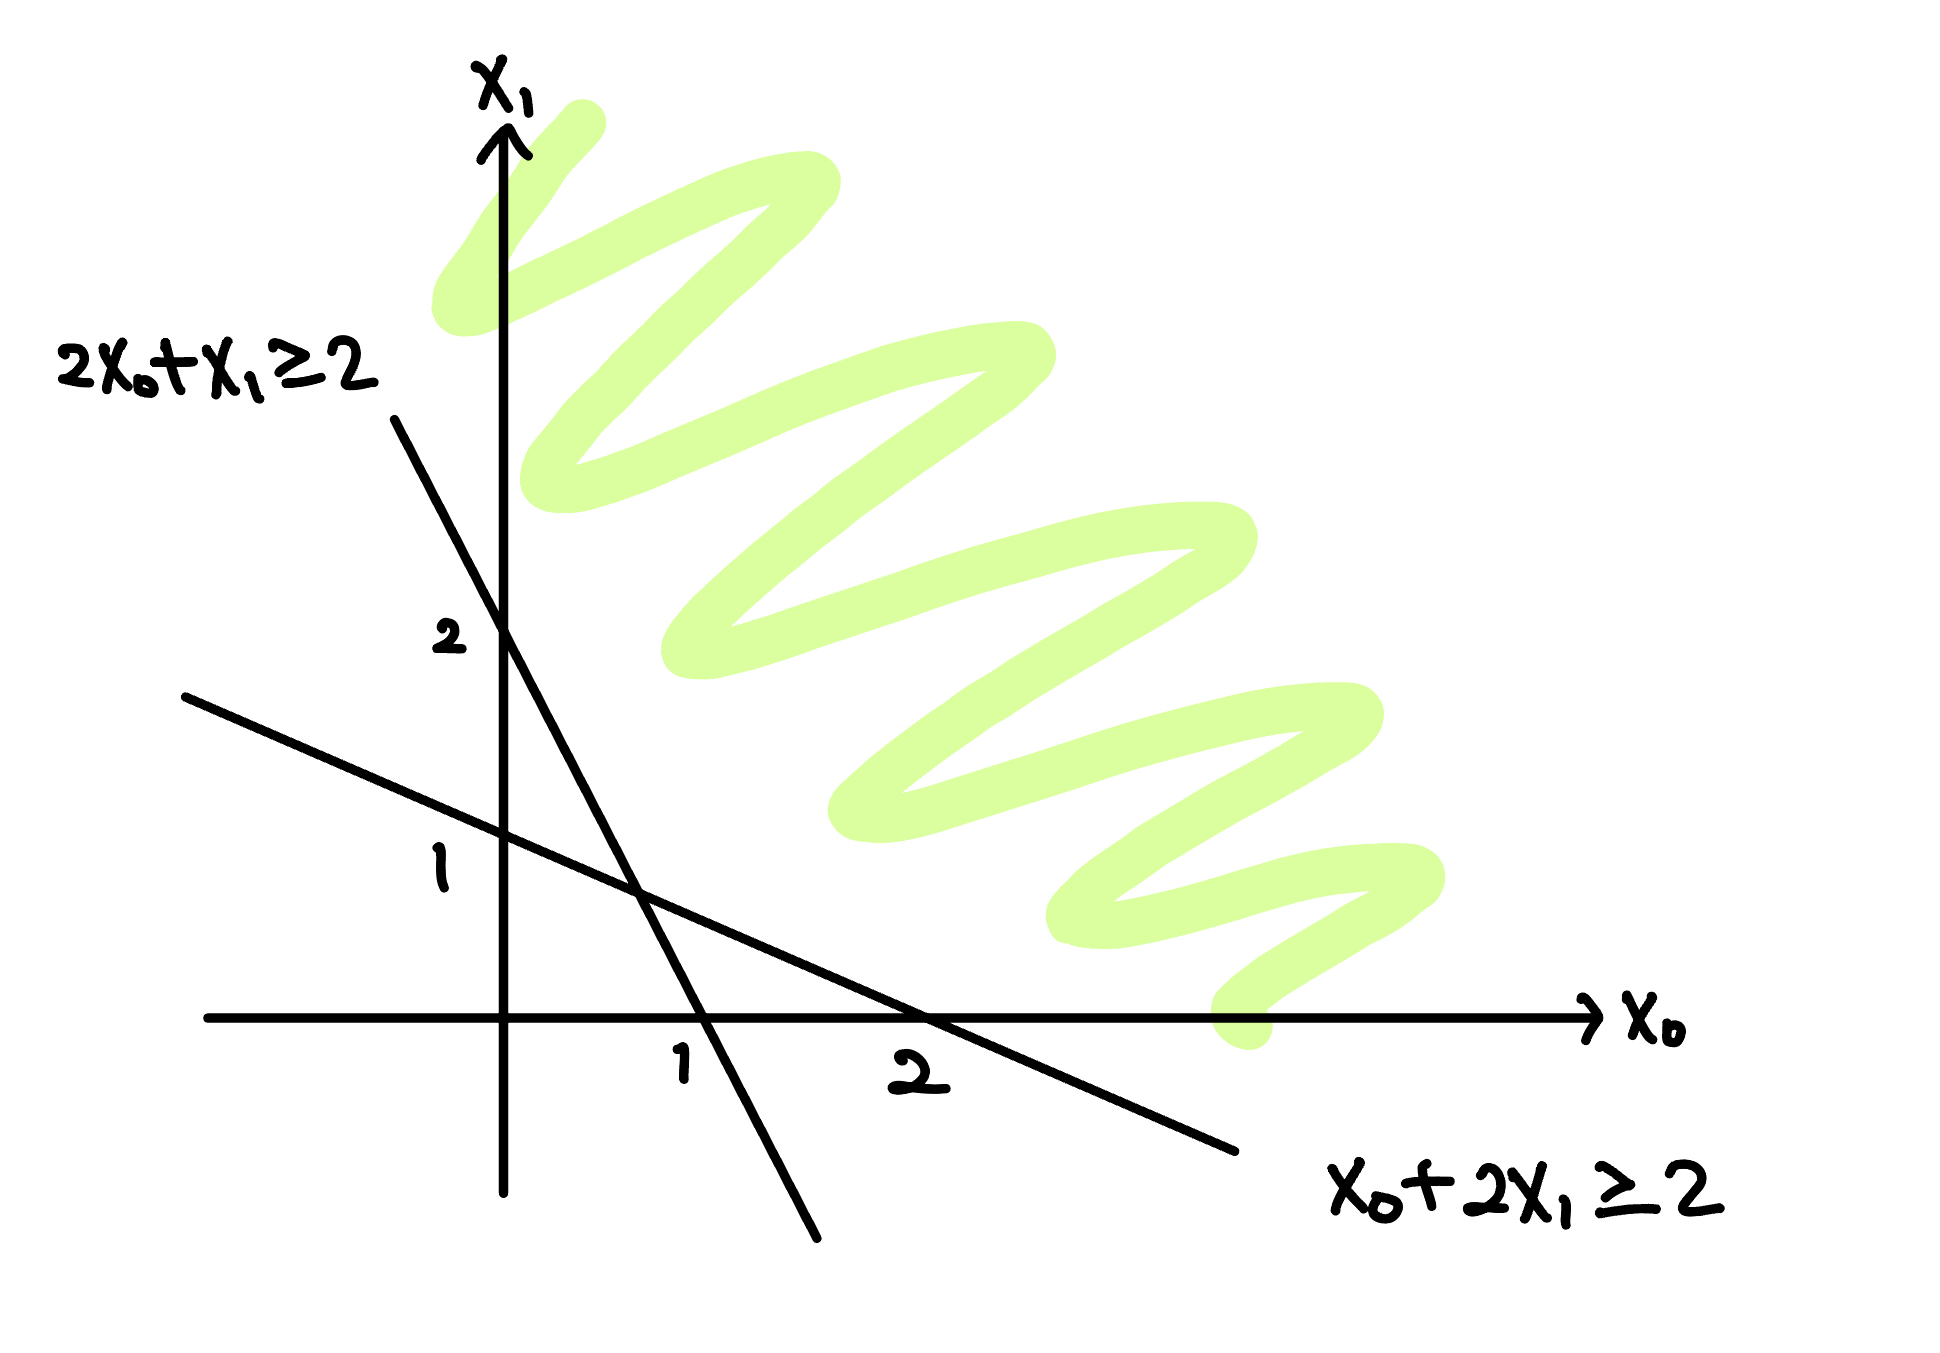
\includegraphics[width=0.6\textwidth]{figure1.png} 

\end{figure}
In this feasible region, the objective function is \textbf{unbounded} hence we cannot get an optimal solution.

\end{solution}
\subsection{}
\begin{solution}
  No, it is still \textbf{possible} for a linear programming problem with an unbounded 
  feasible region to still have an optimal solution. Let's consider the previous example with a slight difference,
\[
    \begin{aligned}
      \text{minimize } &x_0 + x_1 \\ 
      \text{subject to } &2x_0 + x_1 \ge 2 \\ 
                        &x_0 +2x_1 \ge 2 \\ 
                        &x_0,x_1 \ge 0
    \end{aligned}
  \]

  Let's describe the feasible region and the optimal solution of the example above,
  \begin{figure}[H]
\centering
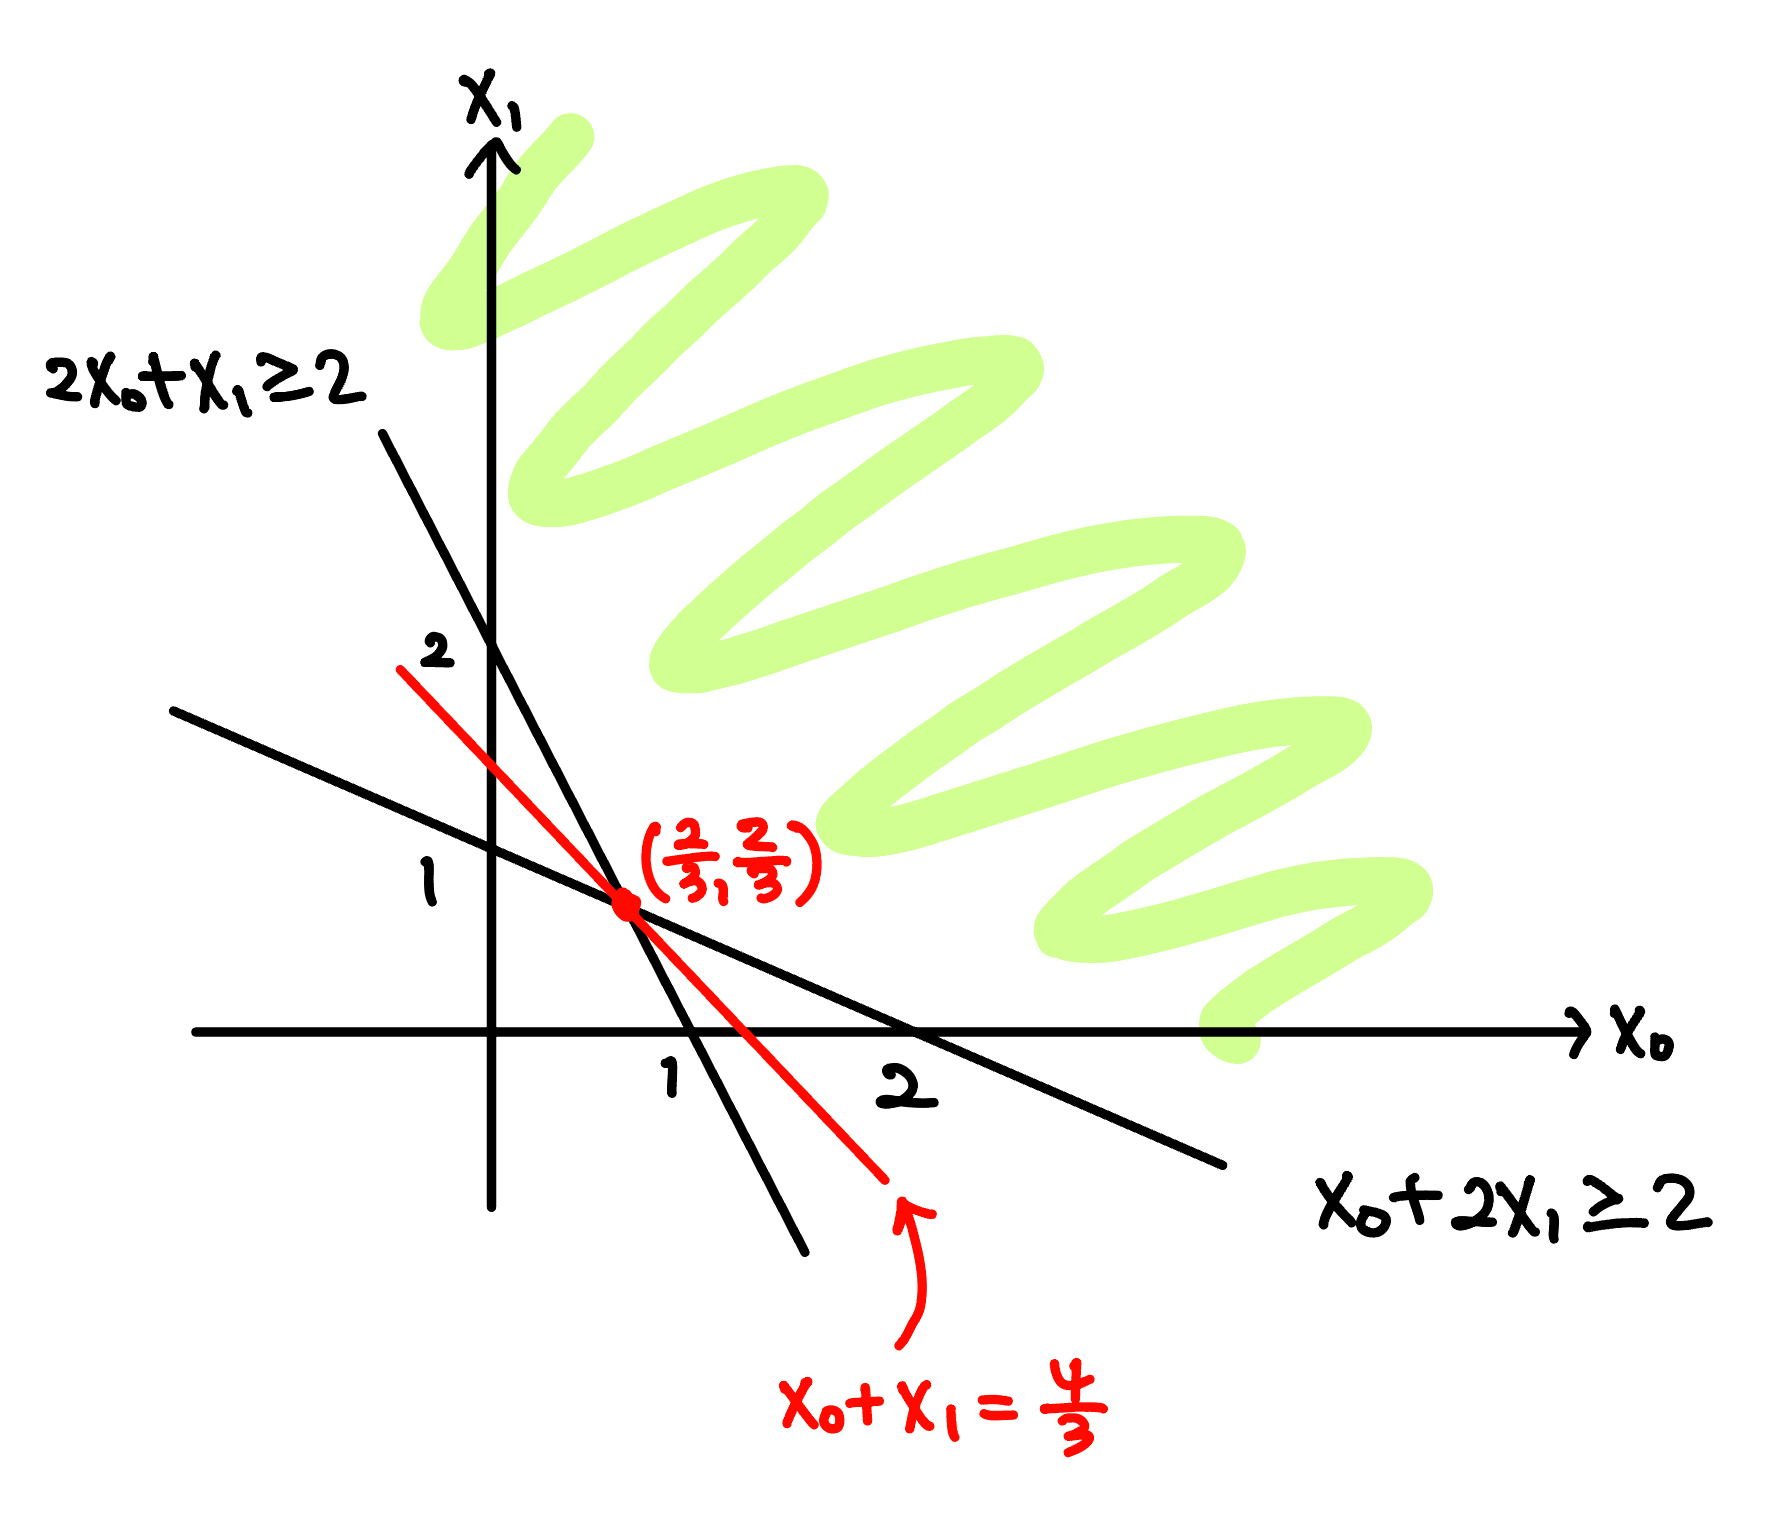
\includegraphics[width=0.6\textwidth]{figure2.png} 
\end{figure}
Since we're getting the minimum, the optimal value (the minimum) can be represented as the red vertex shown. Thus, showing that linear programming problems with an unbounded feasible region can still have an optimal solution.


\end{solution}
\pagebreak

\section*{Question 3}
\begin{solution}
  First, let's determine the ending and leaving variables of 
\[
  \begin{aligned}
    z &= 7-x_1+2x_4 \\ 
    x_2 &= 12 + x_1 - x_4 \\ 
    x_3 &= 5 + x_1 -x_4 \\ 
    x_5 &= 4 +x_1 -x_4
  \end{aligned}
\]
The entering variable in this iteration is $x_4$ since it has the largest positive coefficient of 2. 
By setting $x_1=0$ and observing the behaviour of the basic variables $x_2,x_3,x_5$. We can see that $x_5$ becomes 0 first as $x_4$ increases.
Then,
\[
  \begin{aligned}
    x_5 = 4 + x_1 -x_4 &\to x_4 = 4 + x_1 -x_5 \\ 
    x_2 = 12 + x_1 - x_4 &\to x_2 = 12 + x_1 - (4 + x_1 - x_5) = 8 +x_5 \\ 
    x_3 = 5 + x_1 -x_4 &\to x_3 = 5 + x_1 - (4+x_1-x_5) = 1 + x_5 \\ 
    z = 7 - x_1 + 2x_4 &\to z = 7-x_1 +2x_4 = 7 - x_1 + 2(4+x_1-x_5) = 15 +x_1 -2x_5
  \end{aligned}
\]

Hence, we obtain the new dictionary,
\[
  \begin{aligned}
    z &= 15+x_1 - 2x_5 \\ 
    x_2 &= 8 + x_5  \\ 
    x_3 &= 1+x_5 \\ 
    x_4 &= 4+x_1-x_5
  \end{aligned}
\]
\end{solution}



\section*{Question 4}

\subsection{}
\begin{solution}
  We start with the initial dictionary by introducing slack variables $x_4,x_5,x_6 \ge 0$,
  \[
    \begin{aligned}
      z &= 2x_1+3x_2+3x_3 \\
      x_4 &= 60 -3x_1 -x_2 \\ 
      x_5 &= 10 +x_1 - x_2 -4x_3 \\ 
      x_6 &= 15 - 2x_1 + 2x_2 - 5x_3
    \end{aligned}
  \]
  with,
\[
  \begin{aligned}
    \text{basic variables: } &x_4,x_5,x_6 \\ 
    \text{non-basic variables: } &x_1,x_2,x_3 \\ 
    \text{basic solution: } &(x_1,x_2,x_3,x_4,x_5,x_6) = (0,0,0,60,10,15) \text{ feasible!}
  \end{aligned}
\]
Following Anstee's rule, we can determine that $x_2$ is the entering variable since it has the largest positive coefficient with the smaller subscript.
Also, when setting $x_1=x_3=0$ and increasing $x_2$, we can see that $x_5$ reaches 0 first, hence the leaving variable. 
\[
  \begin{aligned}
    x_4 &= 60 -x_2 \to \text{ 0 at }x_2 = 60\\ 
    x_5 &= 10 -x_2 \to \text{ 0 at }x_2 = 10 \\ 
    x_6 &= 15 + x_2 \text{ never zero} 
  \end{aligned}
\]
\\
Now, let's apply the changes,
\[
  \begin{aligned}
    x_5 = 10 + x_1 -x_2 - 4x_3 &\to x_2= 10 + x_1 -4x_3 - x_5 \\ 
    x_4 = 60-3x_1-x_2 &\to x_4 = 60-3x_1 - (10+x_1-4x_3-x_5) = 50 -4x_1 + 4x_3 +x_5 \\ 
    x_6 = 15-2x_1+2x_2-5x_3 &\to x_6 =  15-2x_1 +2(10+x_1-4x_3-x_5) -5x_3 = 35 -13x_3 -2x_5 \\ 
    z = 2x_1+3x_2+3x_3 &\to z = 2x_1 +3(10+x_1-4x_3-x_5) +3x_3 = 30 + 5x_1 -9x_3 -3x_5 
  \end{aligned}
\]
Which gives us the new dictionary,
\[
  \begin{aligned}
    z &= 30+5x_1-9x_3-3x_5 \\ 
    x_2 &= 10+x_1-4x_3-x_5 \\ 
    x_4 &= 50-4x_1+4x_3 + x_5 \\ 
    x_6 &= 35-13x_3-2x_5
  \end{aligned}
\]
\[
  \begin{aligned}
    \text{basic variables: } &x_2,x_4,x_6 \\ 
    \text{non-basic variables: } &x_1,x_3,x_5 \\ 
    \text{basic solution: } &(x_1,x_2,x_3,x_4,x_5,x_6) = (0,10,0,50,0,35) \text{ feasible!}
  \end{aligned}
\]
In this dictionary, the entering variable is $x_1$ since it is the only one with a positive coefficient. Now, let's set $x_3=x_5=0$, 
if we increase $x_1$, $x_2$ is unbounded, $x_6$ doesn't change, hence $x_4$ is the leaving variable since it reaches zero at $x_1=12.5$.
\[
  \begin{aligned}
    x_2 &= 10 +x_1 \text{ never 0}\\ 
    x_4 &= 50-4x_1 \to \text{ 0 at }x_1=12.5\\ 
    x_6 &= 35 \text{ never 0}
  \end{aligned}
\]
Then,
\[
  \begin{aligned}
    x_4 = 50-4x_1+4x_3 + x_5 &\to x_1 = 12.5 +x_3 -0.25x_4 + 0.25x_5 \\ 
    x_2 = 10+x_1-4x_3-x_5 &\to x_2 = 10 + (12.5 +x_3 -0.25x_4 + 0.25x_5) -4x_3 -x_5\\ 
    &\to x_2 = 22.5 -3x_3 -0.25x_4 -0.75x_5 \\ 
    x_6 = 35-13x_3-2x_5 &\to x_6  = 35-13x_3-2x_5 \\ 
    z = 30 + 5x_1 - 5x_3 -3x_5 &\to z = 30 +5(12.5+x_3 -0.25x_4 +0.25x_5) - 9x_3-3x_5 \\ 
                               &\to z = 92.5-4x_3 -1.25x_4 -1.75x_5 
  \end{aligned}
\]

Ending up with our final dictionary,
\[
  \begin{aligned}
    z &= 92.5-4x_3 -1.25x_4 -1.75x_5 \\ 
    x_1 &= 12.5 +x_3 -0.25x_4 + 0.25x_5 \\ 
    x_2 &= 22.5 -3x_3 -0.25x_4 -0.75x_5 \\
    x_6 &= 35-13x_3-2x_5
  \end{aligned}
\]
And this has a good expression of the objective function. When $x_4=x_5=x_3=0$, 
\[ x_1 = 12.5  \quad x_2 = 22.5  \quad x_6 = 35 \]
\[
  \begin{aligned}
    \text{optimal solution } &(x_1,x_2,x_3,x_4,x_5,x_6) = (12.5 , 22.5,,0,0,35) \to (x_1,x_2,x_3) = (12.5,22.5,0) \\ 
    \text{optimal value: } &92.5
  \end{aligned}
\]
\end{solution}

\subsection{}
\begin{solution}
  Let's construct the initial dictionary by introducing slack variables $x_4,x_5,x_6 \ge 0$,
  \[
  \begin{aligned}
    z &= 3x_1+2x_2+4x_3 \\ 
    x_4 &= 4-x_1-x_2-2x_3 \\ 
    x_5 &= 5-2x_1-3x_3 \\ 
    x_6 &= 7 - 2x_1 - x_2 -3x_3
  \end{aligned}
  \]
\[
  \begin{aligned}
    \text{basic variables: } &x_4,x_5,x_6 \\ 
    \text{non-basic variables: } &x_1,x_2,x_3 \\ 
    \text{basic solution: } &(x_1,x_2,x_3,x_4,x_5,x_6) = (0,0,0,4,5,7) \text{ feasible!}
  \end{aligned}
\]
We can determine that $x_3$ is the entering variable (largest positive coefficient). Given that $x_1=x_2=0$, we can also see that $x_5$ is the leaving variable.
\[
\begin{aligned}
  x_4 &= 4-2x_3 \to \text{ 0 at }x_3=2 \\ 
  x_5 &= 5 -3x_3 \to \text{0 at }x_3 = \frac{5}{3}\\ 
  x_6 &= 7-3x_3 \to \text{ 0 at }x_3 = \frac{7}{3}
\end{aligned}
\]
\[
  \begin{aligned}
    x_5 = 5-2x_1-3x_3 &\to x_3 = \frac{5}{3} -\frac{2}{3}x_1 - \frac{1}{3}x_5 \\ 
    x_4 = 4-x_1 -x_2 -2x_3 &\to x_4 = 4-x_1-x_2 -2(\frac{5}{3} -\frac{2}{3}x_1 - \frac{1}{3}x_5) \\ 
                           &\to x_4 = \frac{2}{3} +\frac{1}{3} x_1 -x_2 + \frac{2}{3}x_5 \\ 
    x_6 = 7-2x_1-x_2-3x_3 &\to x_6 = 7 - 2x_1 -x_2 -3(\frac{5}{3} -\frac{2}{3}x_1 - \frac{1}{3}x_5) \\ 
                          &\to x_6 = 2-x_2+x_5 \\ 
    z=3x_1+2x_2+4x_3 &\to z=3x_1+2x_2+4(\frac{5}{3} -\frac{2}{3}x_1 - \frac{1}{3}x_5) \\ 
                     &= \frac{20}{3} + \frac{1}{3}x_1  +2x_2 -\frac{4}{3}x_5
  \end{aligned}
\]

Our new dictionary is,
  \[
  \begin{aligned}
    z &= \frac{20}{3} + \frac{1}{3}x_1  +2x_2 -\frac{4}{3}x_5\\ 
    x_3 &= \frac{5}{3} -\frac{2}{3}x_1 - \frac{1}{3}x_5 \\ 
    x_4 &= \frac{2}{3} +\frac{1}{3} x_1 -x_2 + \frac{2}{3}x_5\\ 
    x_6 &= 2-x_2+x_5 
  \end{aligned}
  \]
\[
  \begin{aligned}
    \text{basic variables: } &x_3,x_4,x_6 \\ 
    \text{non-basic variables: } &x_1,x_2,x_5 \\ 
    \text{basic solution: } &(x_1,x_2,x_3,x_4,x_5,x_6) = (0,0,\frac{5}{3},\frac{2}{3},0,2) \text{ feasible!}
  \end{aligned}
\]
In this new dictionary, the entering variable is $x_2$ (largest positive coefficient), and the leaving variable is $x_4$. 

\[ 
  \begin{aligned}
    x_3 &= \frac{5}{3} \\ 
    x_4 &= \frac{2}{3}-x_2 \to \text{ 0 at }x_2 = \frac{2}{3} \\ 
    x_6 &= 2-x_2 \to \text{ 0 at }x_2=2
  \end{aligned}
\]
Then,
\[
  \begin{aligned}
    x_4 = \frac{2}{3} +\frac{1}{3} x_1 -x_2 + \frac{2}{3}x_5 &\to x_2 = \frac{2}{3} +\frac{1}{3} x_1 -x_4 + \frac{2}{3}x_5 \\  
    x_3 = \frac{5}{3} -\frac{2}{3}x_1 - \frac{1}{3}x_5 &\to  x_3 = \frac{5}{3} -\frac{2}{3}x_1 - \frac{1}{3}x_5  \\
    x_6 = 2-x_2 +x_5 &\to x_6 = 2-(\frac{2}{3} +\frac{1}{3} x_1 -x_4 + \frac{2}{3}x_5) + x_5 \\ 
                     &\to x_6 = \frac{4}{3} -\frac{1}{3}x_1 +x_4 + \frac{1}{3}x_5  \\ 
    z = \frac{20}{3} + \frac{1}{3}x_1  +2x_2 -\frac{4}{3}x_5 &\to z = \frac{20}{3} + \frac{1}{3}x_1  +2(\frac{2}{3} +\frac{1}{3} x_1 -x_4 + \frac{2}{3}x_5) -\frac{4}{3}x_5 \\ 
                                                             &\to z=  8 +x_1 -2x_4
  \end{aligned}
\]

Hence, our new dictionary is,
  \[
  \begin{aligned}
    z &=  8 +x_1 -2x_4 \\
    x_2 &= \frac{2}{3} +\frac{1}{3} x_1 -x_4 + \frac{2}{3}x_5 \\ 
    x_3 &= \frac{5}{3} -\frac{2}{3}x_1 - \frac{1}{3}x_5 \\
    x_6 &= \frac{4}{3} -\frac{1}{3}x_1 +x_4 + \frac{1}{3}x_5
  \end{aligned}
  \]
\[
  \begin{aligned}
    \text{basic variables: } &x_2,x_3,x_6 \\ 
    \text{non-basic variables: } &x_1,x_4,x_5 \\ 
    \text{basic solution: } &(x_1,x_2,x_3,x_4,x_5,x_6) = (0,\frac{2}{3},\frac{5}{3},0,0,\frac{4}{3}) \text{ feasible!}
  \end{aligned}
\]

Now, again, let's decide the entering and leaving variables. From the coefficients of the objective function, $x_1$ is our entering variable. And consequently, $x_3$ is our leaving variable.
\[
  \begin{aligned}
    x_2 &= \frac{2}{3} +\frac{1}{3}x_1 \text{ never 0} \\ 
    x_3 &= \frac{5}{3} -\frac{2}{3}x_1 \to \text{ 0 at }x_1=\frac{5}{2}  \\ 
    x_6 &= \frac{4}{3} -\frac{1}{3}x_1 \to \text{ 0 at }x_1=4
  \end{aligned}
\]
Then,
\[
  \begin{aligned}
    x_3 = \frac{5}{3} -\frac{2}{3}x_1 - \frac{1}{3}x_5 &\to x_1 = \frac{5}{2} -\frac{3}{2}x_3 - \frac{1}{2}x_5   \\ 
    x_2 =  \frac{2}{3} +\frac{1}{3} x_1 -x_4 + \frac{2}{3}x_5 &\to x_2 =  \frac{2}{3} +\frac{1}{3} (\frac{5}{2} -\frac{3}{2}x_3 - \frac{1}{2}x_5) -x_4 + \frac{2}{3}x_5 \\ 
                                                              &\to x_2 = \frac{3}{2} -\frac{1}{2}x_3 -x_4 +\frac{1}{2}x_5 \\ 
    x_6 = \frac{4}{3} -\frac{1}{3}x_1 +x_4 + \frac{1}{3}x_5 &\to x_6 = \frac{4}{3} -\frac{1}{3}(\frac{5}{2} -\frac{3}{2}x_3 - \frac{1}{2}x_5) +x_4 + \frac{1}{3}x_5 \\ 
                                                            &\to x_6 =  \frac{1}{2} +\frac{1}{2}x_3 +x_4 +  \frac{1}{2}x_5 \\ 
    z = 8 +x_1 -2x_4 &\to z = 8 + (\frac{5}{2} -\frac{3}{2}x_3 - \frac{1}{2}x_5) -2x_4 \\ 
                     &\to z= \frac{21}{2} -  \frac{3}{2}x_3-2x_4 - \frac{1}{2}x_5
  \end{aligned}
\]
Therefore, giving the new dictionary in a "good" form,
 \[
  \begin{aligned}
    z &=  \frac{21}{2} -  \frac{3}{2}x_3-2x_4 - \frac{1}{2}x_5\\
    x_1 &= \frac{5}{2} -\frac{3}{2}x_3 - \frac{1}{2}x_5  \\ 
    x_2 &= \frac{3}{2} -\frac{1}{2}x_3 -x_4 +\frac{1}{2}x_5 \\
    x_6 &= \frac{1}{2} +\frac{1}{2}x_3 +x_4 +  \frac{1}{2}x_5 
  \end{aligned}
  \]
When $x_3=x_4= x_5=0$, we get the optimal solution and value,

\[
  \begin{aligned}
    \text{optimal solution: } &(x_1,x_2,x_3,x_4,x_5,x_6) = (\frac{5}{2},\frac{3}{2},0,0,0,\frac{1}{2}) \to (x_1,x_2,x_3) = (\frac{5}{2},\frac{3}{2},0) \\ 
    \text{optimal value: } &10.5
  \end{aligned}
\]
\end{solution}

\section*{Question 5}
\begin{solution}
 Let's look at the dictionary,
\[
  \begin{aligned}
    z &= 8+x_1-2x_4+2x_6 \\ 
    x_2 &= 12-x_1 + x_4 + x_6 \\ 
    x_3 &= 1+x_1 + x_6 \\ 
    x_5 &= 4 + x_1 +x_4
  \end{aligned}
\]
If we follow Anstee's rule, $x_6$ is our entering variable since it has the largest positive coefficient. And given this, when saying $x_1=x_4 =0$, we can get the following expressions,
\[
  \begin{aligned}
    x_2 &= 12+x_6 \\ 
    x_3 &= 1+x_6 \\ 
    x_5 &= 4 
  \end{aligned}
\]
We can see that none of $x_2,x_3,x_5$ reach zero as $x_6$ increases. In other words, we have that $x_2,x_3$ are unbounded in the feasible region. 
If we observe the objective function with the increasing $x_6$,
\[ z = 8+2x_6 \]
$z$ will also increase without a bound while the constraints are still satisfied. Hence, we can conclude that the linear programming problem is unbounded and there is no optimal solution in this case.
\end{solution}

\end{document}
